\section{Decays and reactions}
\label{sec:DecaysAndReaction}
In particle physics we are interested in particle decays and interactions ie transitions between states.
\subsection{Decays}
Lets define the probability per unit time that a decay occurs as $\Gamma$, that is
\begin{equation}
\frac{dP}{dt}=\Gamma
\end{equation}
If the probability for NO decay to occur within time $t$ is denoted by $P(0;t)$, then the probability of NO decay until time $t+dt$ is given by the product of $P(0;t)$ and the probability of NO decay in interval $dt$, ie
\begin{equation}
P(0;t+dt)=P(0;t)(1-\Gamma dt)
\end{equation}
rearranging we get
\begin{equation}
P(0;t+dt)-P(0;t)=-P(0;t)\Gamma dt
\end{equation}
therefore
\begin{equation}
\frac{dP(0;t)}{dt}=-P(0;t)\Gamma
\end{equation}
So we have that:
\begin{equation}
P(0;t)=Ae^{-\Gamma t}
\end{equation}
Using the initial condition at the probability to survive at $t=0$ is 1, we have that 
\begin{equation}
P(0;t)=e^{-\Gamma t}
\end{equation}
However we said that $P(0;t)$ denotes a probability so we need to make sure that it is correctly normalised such that $\int_{0}^{\infty} P(0;t)=1$. Therefore
\begin{eqnarray*}
N\int_{0}^{\infty}e^{-\Gamma t}=1 \therefore
N=\Gamma
\end{eqnarray*}
So we finally have
\begin{equation}
P(0;t)=\Gamma e^{-\Gamma t}
\end{equation}
We can also calculate the average expected time before a decay occurs 
\begin{equation}
<t>\equiv\tau=\int_{0}^{\infty}P(0;t)tdt=\frac{1}{\Gamma}
\end{equation}
So we can write:
\begin{equation}
P(0;t)=\frac{1}{\tau} e^{-t/\tau}
\end{equation}
Now we can wave our hands a little bit and relate $\Gamma$ with mass. How? We can use the uncertainty principle $\Delta t\Delta E\geq \hbar/2$. So for particles with short life-time, their energy (mass) will be badly defined. So can think of $\Gamma$ as $\Delta E$, or in other words as the width of the mass distribution of the particle
\begin{center}
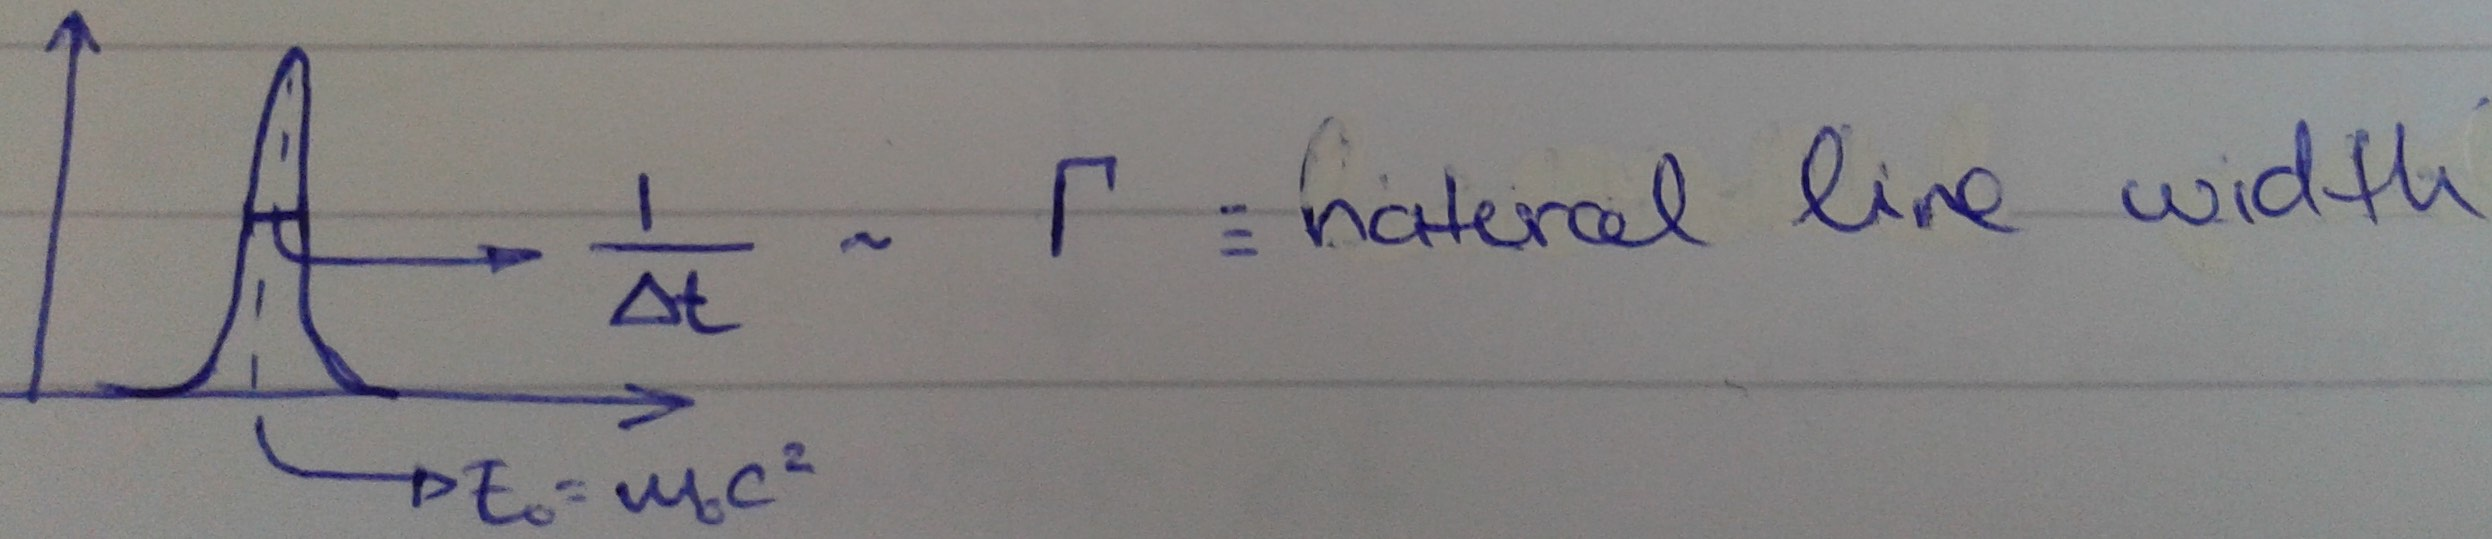
\includegraphics[width=0.7\textwidth]{fig/decaysreactions/particle_width.jpg}
\end{center}

What is more, instead of asking for the probability for a decay to occur, can ask for the probability for a decay to a particular state out of many, to occur. So we can define a partial lifetime $\tau_i$ and partial width $\Gamma_i$ such that
\begin{equation}
\Gamma=\sum_{i}\Gamma_i
\end{equation}
Can also define the ``Branching Fraction" ($B_i$) as
\begin{equation}
B_i=\frac{\Gamma_i}{\Gamma}
\end{equation}
with 
\begin{equation}
\sum_{i}B_i=1.
\end{equation}

\subsection{Reactions}

We have discussed the probability of $e^+e^-\to\mu^+\mu^-$ by exchanging a virtual photon between the initial and final states. We have also said that the probability for such a process is proportional to the fine structure constant squared $\alpha_{EM}^2$ or in other words proportional to the charge of the electron to the fourth power. However this is not the full picture.

Consider the collision between an $e^+$ and an $e^-$ beam . The interaction rate depends on the beam intensity and density of particles in the beam, as well as the strength of the interaction (ie the type of force involved in the interaction). We therefore define the cross-section 
$\sigma$ of a process (eg $ee\to\mu\mu$)  on 
\begin{equation}
\sigma=\frac{|M_{fi}|^2}{({\rm beam\,\,\,flux})}\times({\rm Energy\,\,\,available\,\,\,in\,\,\,interaction}),
\end{equation}
where $M_{fi}$ is the matrix element of the transition from an initial state $i$ to a final state $f$. The magnitude square of the matrix element is associated to the probability of the transition to occur. For $ee\to\mu\mu$ this probability is proportional to $e^4$. For the full expression, you need to wait until next year. The ``beam flux" is the number of incident particles per unit time per unit area and the ``Energy available in interaction'' is also called the phase-space of the interaction. The cross-section can be thought as an effective cross-sectional area of the target particles for the interaction to occur. Though in general, it has nothing to do with the physical size of the target!!!

